\documentclass[tikz,border=10pt]{standalone}
\usetikzlibrary{shapes.geometric, positioning, arrows.meta, scopes, patterns, shadows, calc}
\usepackage{xstring}

\def\code#1{\color{olive}{\texttt{#1}}\color{black}~}
% \def\refer#1{Fig. \ref{#1}}
% \newcommand{\urlpath}[1]{%
% \begin{FVerbatim}[fontsize=\scriptsize]
% #1
% \end{FVerbatim}%
% }

\def\comment#1{\color{olive}{\textit{\% #1}} \color{black}}

\newcommand\ezeq[1]{$#1$}

\newcommand\ezcolumn[3]{
\begin{column}{#1\textwidth}
    \vspace{#2cm}
    #3
\end{column}
}

% \newenvironment{myenumerate}{%
%   \begin{enumerate}
%     \renewcommand{\theenumii}{\arabic{enumi}.\arabic{enumii}}
%   }
%   {%
%   \end{enumerate}
% }


\newcommand{\customenumerate}{%
  \renewcommand{\theenumii}{\arabic{enumi}.\arabic{enumii}}
  \renewcommand{\theenumiii}{\arabic{enumi}.\arabic{enumii}.\arabic{enumiii}}
}


\begin{document}
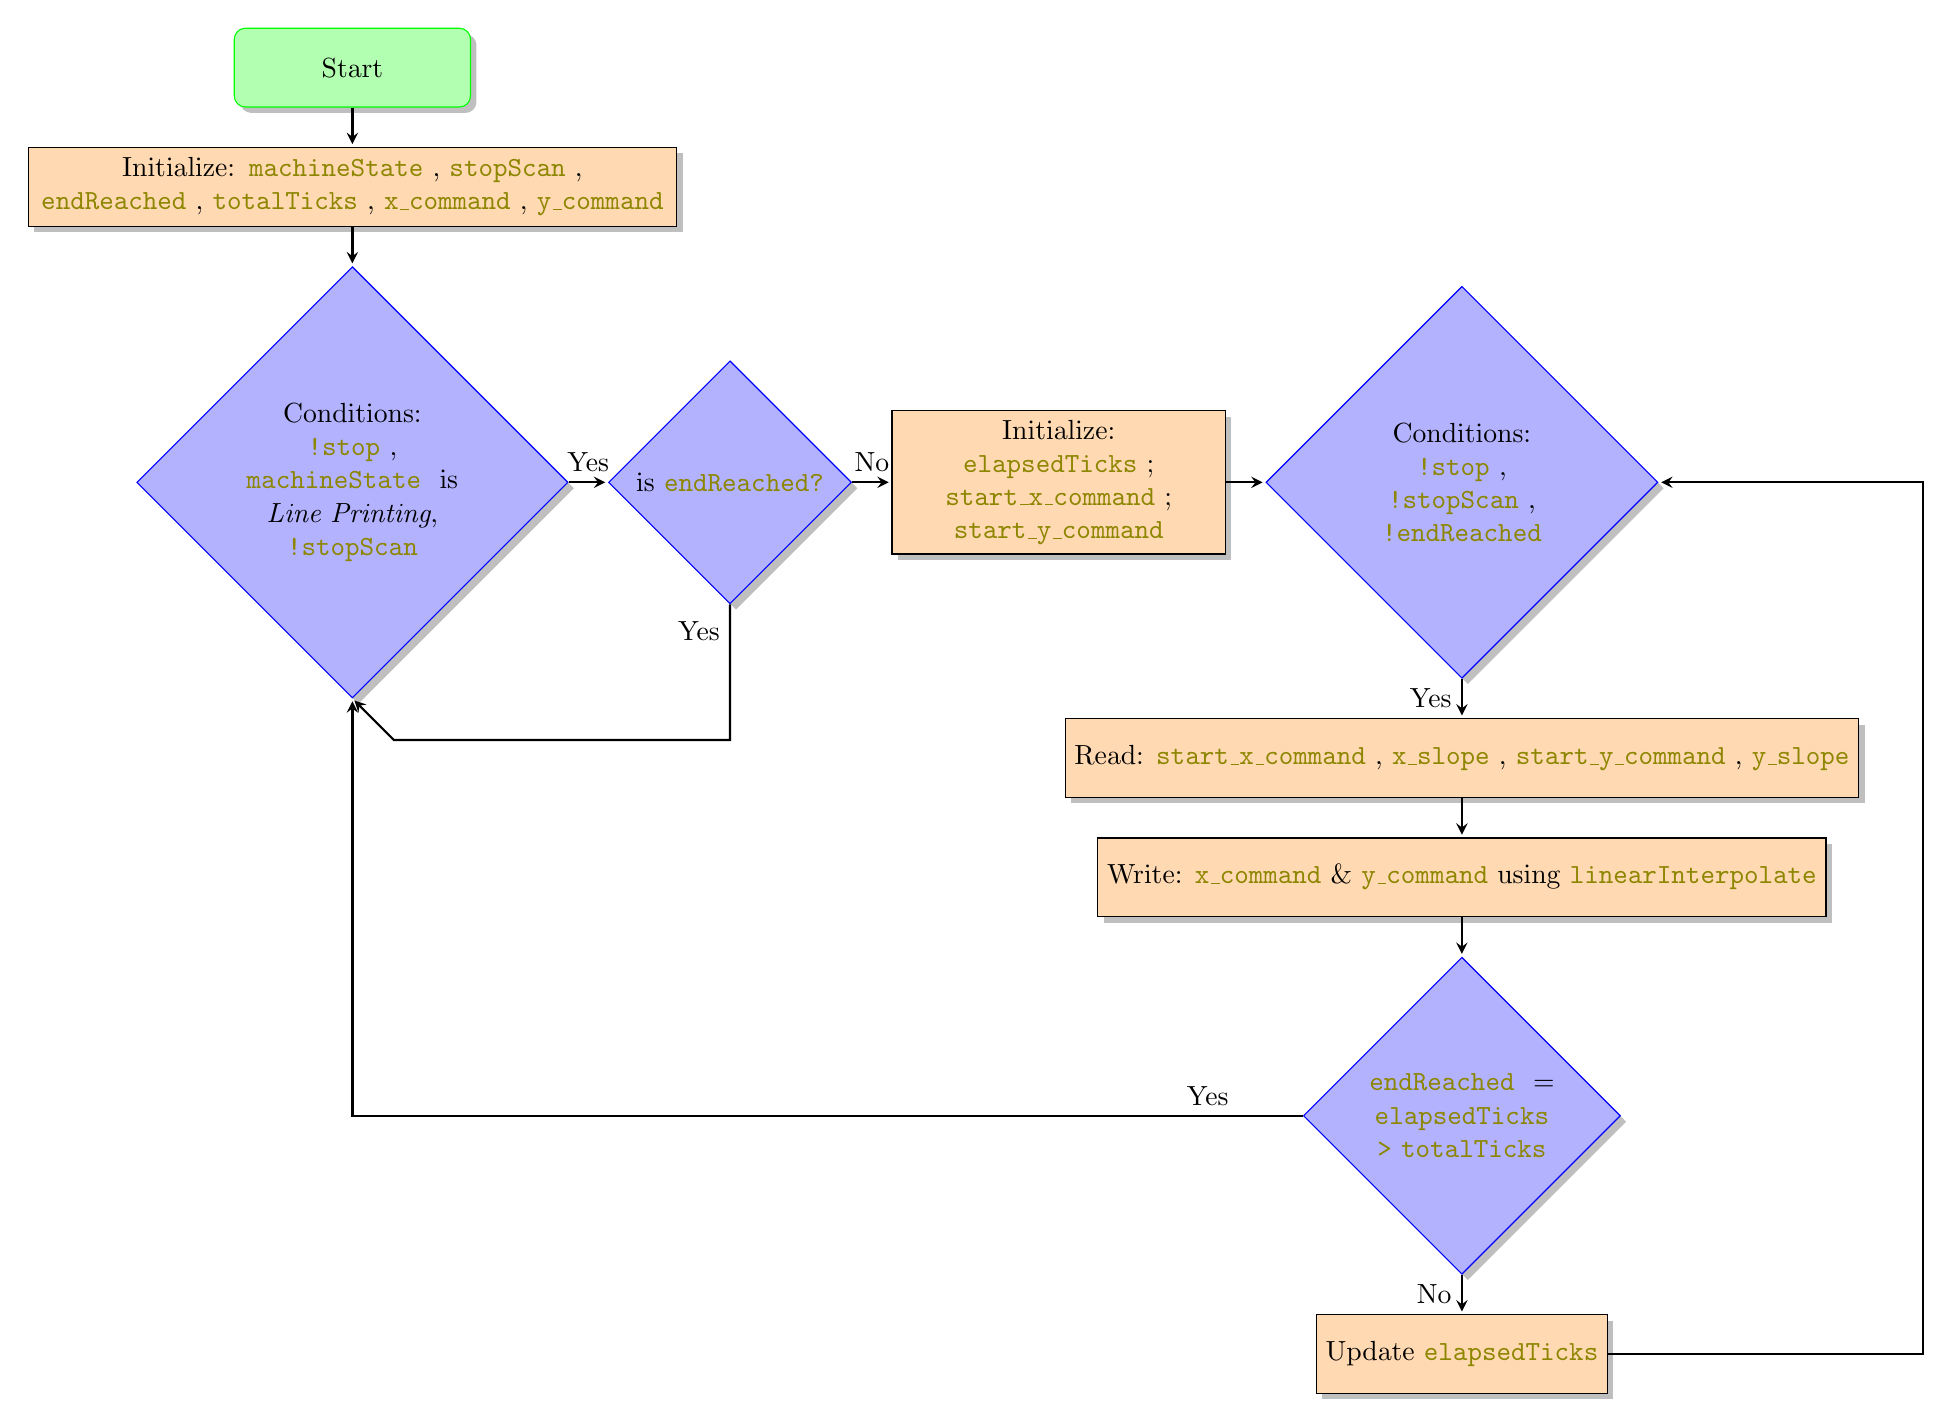
\begin{tikzpicture}[
    startstop/.style={rectangle, rounded corners, minimum width=3cm, minimum height=1cm, text centered, draw=green, fill=green!30, drop shadow},
    process/.style={rectangle, minimum width=3cm, minimum height=1cm, text centered, draw=black, fill=orange!30, drop shadow},
    io/.style={trapezium, trapezium left angle=70, trapezium right angle=110, minimum width=3cm, minimum height=1cm, text centered, draw=blue, fill=blue!30, drop shadow},
    decision/.style={diamond, minimum width=3cm, minimum height=1.5cm, text centered, draw=blue, fill=blue!30, drop shadow},
    arrow/.style={thick,->,>=stealth, shorten >=1pt},
]

% Initial definitions
\node (start) [startstop] {Start};
\node (init1) [process, below=0.5cm of start, text width=8cm] {Initialize: \code{machineState}, \code{stopScan}, \code{endReached}, \code{totalTicks}, \code{x\_command}, \code{y\_command}};
\node (outerCheck) [decision, below=0.5cm of init1, text width=3cm, align=center] {Conditions: \code{!stop}, \code{machineState} is \textit{Line Printing}, \code{!stopScan}};
\node (initCheckEnd) [decision, right=0.5cm of outerCheck] {is \code{endReached?}};
\node (init2) [process, right=0.5cm of initCheckEnd, text width=4cm] {Initialize: \code{elapsedTicks}; \code{start\_x\_command}; \code{start\_y\_command}};
\node (innerCheck) [decision, right=0.5cm of init2, text width=3cm, align=center] {Conditions: \code{!stop}, \code{!stopScan}, \code{!endReached}};
\node (readValues) [process, below=0.5cm of innerCheck] {Read: \code{start\_x\_command}, \code{x\_slope}, \code{start\_y\_command}, \code{y\_slope}};
\node (writeValues) [process, below=0.5cm of readValues] {Write: \code{x\_command}\& \code{y\_command}using \code{linearInterpolate}};
\node (checkEnd) [decision, below=0.5cm of writeValues, text width=2.5cm, align=center] {\code{endReached} = \code{elapsedTicks > totalTicks}};
\node (computeTick) [process, below=0.5cm of checkEnd] {Update \code{elapsedTicks}};

% Arrows and paths
\draw [arrow] (start) -- (init1);
\draw [arrow] (init1) -- (outerCheck);
\draw [arrow] (outerCheck) -- node[anchor=south] {Yes} (initCheckEnd);
\draw [arrow] (initCheckEnd) -- node[anchor=south] {No} (init2);
\draw [arrow] (init2) -- (innerCheck);
\draw [arrow] (innerCheck) -- node[anchor=east] {Yes} (readValues);
\draw [arrow] (readValues) -- (writeValues);
\draw [arrow] (writeValues) -- (checkEnd);
\draw [arrow] (checkEnd) -- node[anchor=east] {No} (computeTick);

% Looping paths
\draw [arrow] let \p1 = (computeTick.east), \p2 = (innerCheck.east) in 
  (computeTick.east) -- ++(4cm,0) -- (\x1 + 4cm, \y2) -- (\x2, \y2);% \draw [arrow] (innerCheck) -- node[anchor=south] {No} ++(-3cm,0) |- (outerCheck.west);
\draw [arrow] let \p1 = (checkEnd.west), \p2 = (outerCheck.south) in 
  (checkEnd.west) -- node[anchor=south, pos=0.1] {Yes} (\x2, \y1) -- (\x2, \y2);
\draw [arrow] let \p1 = (initCheckEnd.south), \p2 = (outerCheck.south) in 
  (\p1) -- node[pos=0.2, anchor=east] {Yes} (\x1,\y2-15) 
  -- (\x2+15,\y2-15) 
  -- (\p2);
  
\end{tikzpicture}
\end{document}
